\section{Shortcomings With Text-Based Authentication} 

  %\cite{DejaVu}
  User authentication is a central component of security systems. In order to get access to systems you need to pass a authentication process. Despite the large number of options for auentication, text-based passwords remain the most common authentication scheme. The reason why they are widley adopted is because they are easy and inexpensie to implement, and users are familiar with the scheme. It is also avoiding the privacy issues raised by biometrical authentication and avoid the need for bringing a physical security device that are used in token-based authentication schemes. However, text-based authentication suffer from both security and usability disadvatages. Today, users needs to remember an increasinly number of password, making users to adopt bad password habits. 

  The term ``habit'' is often a bad thing when talking about security. A habit is often hard to change and are often a predictable pattern. Password reuse is one of the known password habits among users becuase the human limitation to remembering text-based password. Some users also make simple or meaningful password that are easier to remember, making their passwords vulnerable to attacks.
  It is a well known problem that users tends to have an increasingly number of accounts that requires the users to remember yet another number of password across multiple systems and devices. The problem is not just to remember all the password needed, but also remembering which passwords that belongs to which account or device. Because of the human capacity of remembering password are causing users to choose weak passwords, as well as reuse the passwords across multiple web pages. In order to understand the shortcomings with text-based passwords, this section will include relevant research on users choices on text-based passwords.  

  \begin{wrapfigure}{l}{0.4\textwidth}
    \vspace{-20pt}
    \begin{center}
      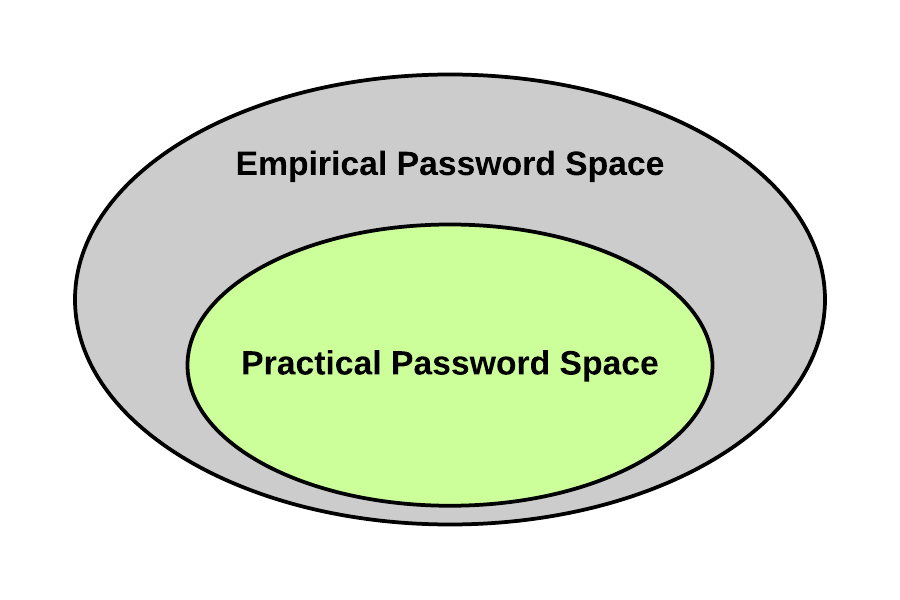
\includegraphics[scale=0.16]{pics/EmpiricalVsPractical.png}
    \end{center}
    \vspace{-20pt}
    \caption{Empirical vs. Practical Password Space}
    \vspace{0pt}
  \end{wrapfigure}

  Password schemes have what is called an empirical password space, that is the number of possible passwords that a user can make. The problem with many password schemes is that it seems that users dont tend to use the full password space, but only a subset of the possible passwords, e.g. the practical password space, making the practical password space less than the empirical password space.

  In a case study of 14.000 Unix passwords, a research group found a 25\% of the passwords were in a group of words forming a dictionary of $3\times10^{6}$ words \cite{UnixPasswords}. This dictionary shows that an attacker can have a relatively high success rate with an attack, despite the fact that there a roughly $2\times10^{14}$ 8-character passwords consisting of digits, and upper case and lower case letters. Due to the limitations of human memory, useres often choose passwords which are easier to remember, causing a significant number of user-chosen password to fall into a small dictionary, e.g. practical password space \cite{Tao}. A well-designed dictionary is a tiny subset of the full password spave, e.g. theoretical password space, which further can be prioritized  according to the likelihood for a password to be chosen. It is therefore a commonly stated that the security of a password scheme is releted closely to the size of its memorable/practical password space, rather than its theoretical password space. 

  One of the first large-scale studies on web password habits was conducted in 2007 by Microsoft research \cite{habits1}. They analyzed web password habits among 544960 web users over a period of 3 months. The data was collected from a Windows Live Toolbar and they observed activities like login frequency. They also collected information about the users age, the strength of the users passwords, as well as number of unique passwords and its use across different URLs. They observed that a normal user have an average of 7 distinct password and that an average of 5 of these password was re-used on different web pages. The estimate on average number of account pr user was estimated to be 25 account pr user, but this would probably be higher since it 7 years ago. 

  {\color{red} \bf WRITE SOMWTHING MORE??}

  %REWRITE!!!
  Because of the shortcomings with text-based authentication, graphical auyhentication are getting getting increased attention becuase it are an alternative to text-based authentication trying to cope with the memorability and security issues of text-based password.
   
